Durante el desarrollo de esta tesis se tuvo la oportunidad de participar en
múltiples proyectos que involucran los temas y técnicas tratados en esta tesis.
El amplio espectro de aplicaciones de las técnicas de \hyperlink{abbr}{IA}, el
rendimiento excepcional de las \hyperlink{abbr}{ConvNets} en tareas de
\hyperlink{abbr}{VC}, la mejora de la eficiencia de los procesos dentro de una
organización al ser vistos desde la perspectiva de las \hyperlink{abbr}{TI} y
\hyperlink{abbr}{SE}s y la facilidad y velocidad del lenguaje Python permitieron
la productividad académica acá expuesta.
 
\subsection{Ponencia en CiLOG 2018}

El Congreso Internacional de Logística y Cadena de Suministro
(\autoref{fig:cilog}), en su edición 2018 fue celebrado en el Palacio de Minería
en la Ciudad de México los días 10 a 12 de Octubre. Surge de los esfuerzos de la
Asociación Mexicana de Logística y Cadena de Suministro para congregar expertos
y estudiantes en el área para divulgar nuevas investigaciones, generar
conocimiento nuevo y vincular investigadores para 

\begin{figure}[H]
    \centering
    
\includegraphics[width=0.6\textwidth]{capitulo_final/cilog}
    \caption{Congreso Internacional de Logística y Cadena de Suministro}\label{fig:cilog}
\end{figure}

Siendo uno de los eventos líderes en su área en América Latina, se tuvo la
fortuna de poder presentar una ponencia basada en el artículo titulado:

\begin{quote}
\textbf{Using Geographical Information Systems to solve Epidemiological and
    Obstetrical Risks within an Organization Health Supply Chain}
\end{quote}

Cuyos autores y afiliaciones fueron:

\begin{itemize}
    \item Marco J. Del Moral-Argumedo -- Tecnológico Nacional de México /
    Instituto Tecnológico de Orizaba
    \item Alberto A. Aguilar-Lasserre -- Tecnológico Nacional de México /
    Instituto Tecnológico de Orizaba
    \item Carlos F. Vázquez-Rodríguez -- IMSS / Coordinación Médica Auxiliar en
    Investigación en Salud
\end{itemize}

Se muestra el abstract o resumen del artículo como referencia:

\begin{quote}
\emph{Abstract—Within the Instituto Mexicano del Seguro Social (IMSS) Delegación
    Veracruz Sur (DVS) over a period of several months maternal deaths have
    occurred due to the dengue fever vector, the mosquito Aedes Aegypti. When a
    pregnant woman arrived, their symptoms were confused with another syndrome
    which the treatment is almost 100\% lethal in pregnant women infected with
    dengue. Mosquito’s behavior is well known so policies can be formulated to
    determine the risk of exposure; knowing this and by thinking treatment
    providing as a supply logistic chain based on the interactions within its
    elements, a paper and ink solution was devised to stop these deaths. Using
    modern software practices and Geographic Information Systems, our solution
    was transformed into a platform to assist decision makers within the IMSS,
    in real time, to evaluate risks such as disease exposure; allowing the
    organization to implement correct logistic policies to deal with
    epidemiological events. The tool can provide passive and active
    epidemiological oversight in both populations to evaluate obstetrical risks.
    Focusing on further objectives, our tool can be extended to create a
    Knowledge Management System that can be applied to the whole organization to
    provide geo epidemiological analysis and prediction. At the current state,
    the platform is fully functional for its intended operational use, our
    implementation applies parallel, asynchronous and distributed computing, and
    is awaiting approval to be implemented in all clinics and hospitals of the
    Instituto Mexicano del Seguro Social (IMSS) Delegación Veracruz Sur (DVS).}
\end{quote}

\subsection{Capítulo de Libro}

Derivado de la ponencia en el congreso, se logró publicar el trabajo presentado
en un libro publicado por la editorial Pearson (\autoref{fig:libro}),
especializada en libros de texto, de divulgación e investigación. La ficha
bibliográfica es la siguiente:

\begin{itemize}
    \item{\textbf{Editores: }} Mauricio Lopez-Acosta,  Jose Manuel
    Velarde-Cantu, Miguel Gaston Cedillo-Campos, Alfredo Bueno-Solano, Ernesto
    Alonso Lagarda-Leyva
    \item{\textbf{Año: }} 2019
    \item{\textbf{Título: }} Gestión en la cadena de suministro: Aplicaciones en
    Latinoamérica
    \item{\textbf{Editorial: }} Pearson.
    \item{\textbf{Lugar: }} Ciudad de México.
    \item{\textbf{ISBN: }} 978-607-32-4878-5.
\end{itemize}

\begin{figure}[H]
    \centering
    
\includegraphics[width=0.3\textwidth]{capitulo_final/libro}
    \caption{Portada}\label{fig:libro}
\end{figure}

El capítulo incluido es el Quinto, en las páginas 67-79. Si bien el tema del
capítulo es igual al de la ponencia, se coloca el título del mismo ya que se
tradujo al español para su publicación:

\begin{quote}
\textbf{Uso de sistemas de información geográfica para resolver riesgos
    epidemiológicos y obstétricos dentro de la cadena de suministros de salud de
    una organización}
\end{quote}

Los autores del capítulo son los mismos del artículo y ponencia presentadas en
el congreso, igualmente se coloca el abstract como referencia al ser traducido
al español:

\begin{quote}
\emph{Dentro del Instituto Mexicano del Seguro Social (IMSS) Delegación Veracruz Sur,
han ocurrido muertes maternas debido al vector del Dengue, el mosquito Aedes
Aegypti. Cuando una mujer embarazada llegaba a la clínica, sus síntomas eran
confundidos por otro síndrome cuyo tratamiento resulta 100\% letal si la mujer
embarazada está infectada. El comportamiento del mosquito es bien conocido así
que se pueden formular políticas para determinar el riesgo de exposición. Usando
prácticas modernas de software y Sistemas de Información Geográfica y pensando
en la provisión de tratamientos como una cadena de suministros basada en las
interacciones entre sus elementos, desarrollamos una plataforma para evaluar
riesgos como la exposición a una enfermedad, permitiendo a la organización
implementar políticas logísticas correctas para solucionar eventos
epidemiológicos. La plataforma puede proveer vigilancia epidemiológica pasiva y
activa en ambas poblaciones para evaluar el riesgo obstétrico. Enfocándonos en
objetivos ulteriores, nuestra herramienta puede ser extendida para crear un
Sistema de Gestión del Conocimiento que puede ser aplicado a toda la
organización para proveer análisis geo-epidemiológico y predicción. En su estado
actual, la plataforma es totalmente funcional, aplica cómputo en paralelo,
asíncrono y distribuido y se encuentra esperando aprobación para ser
implementado en todas las clínicas y hospitales del IMSS.}
\end{quote}

\subsection{Estancia Internacional de Investigación}

Se realizó una estancia de investigación de tres meses de duración, Junio -
Agosto 2019, en Toulouse, Francia; en el Laboratorio de Ingeniería Química del
Instituto Nacional Politécnico (\autoref{fig:estancia}) bajo la tutela de la
\textbf{Doctora Catherine Azzaro-Pantel}, experta en optimización matemática y
metaheurísticas.

\begin{figure}[H]
    \centering
    \begin{subfigure}{.49\textwidth}
        \centering
        
\includegraphics[width=.6\linewidth]{capitulo_final/lgc}
        \caption{Laboratorio de Ingeniería Química}
    \end{subfigure}%
    \begin{subfigure}{.5\textwidth}
        \centering
        
\includegraphics[width=.7\linewidth]{capitulo_final/inp}
        \caption{Instituto Nacional Politécnico}
    \end{subfigure}
    \caption{Instituciones francesas de la estancia}\label{fig:estancia}
\end{figure}

En esta estancia se trabajó con la rama de \hyperlink{abbr}{IA} de los
\emph{Algoritmos Evolutivos}, que son algoritmos inspirados en la naturaleza
capaz de evolucionar soluciones que den el mejor resultado posible (máximo o
mínimo) de una función o modelo matemático. En concreto, se utilizó el algoritmo
\emph{NSGA2} (capaz de optimizar múltiples criterios al mismo tiempo) para
evolucionar hiperparámetros que optimicen el rendimiento ya sea maximizando
exactitud o minimizando pérdida, de una \hyperlink{abbr}{ConvNet} aplicada a un
problema de \hyperlink{abbr}{VC}.

Los resultados del experimento fueron sumamente prometedores. PSe maximizó la
exactitud, representada en la \autoref{fig:resultnsga} como el eje \(z\) y se
tomaron dos criterios: la tasa de aprendizaje (eje \(y\)) y el número de neuronas
(eje \(x\)) representado por un número entero que resuelve la ecuación \(2^{n}\). Se
puede observar que el algoritmo encontró soluciones que consistentemente se
aproximaban al óptimo de la exactitud y no solo ello, sino encontrando
soluciones excelente con modelos menos complejos; como se expuso anteriormente
en esta tesis, se favorecen siempre los modelos menos complejos debido a que son
capaces de generalizar mejor.

\begin{figure}[H]
    \centering
    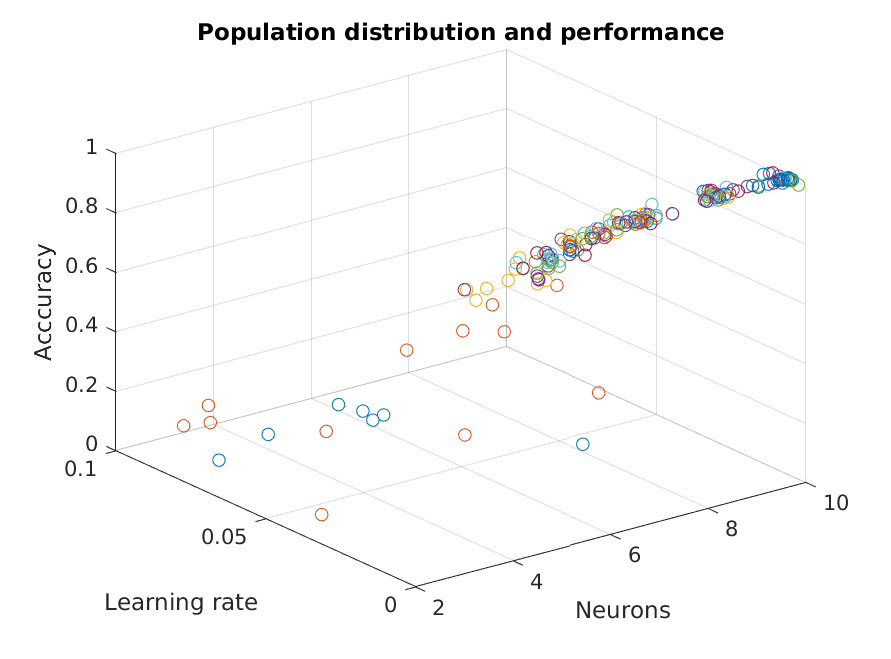
\includegraphics[width=0.6\textwidth]{capitulo_final/scatter3}
    \caption{Resultados del experimento con \emph{NSGA2}}\label{fig:resultnsga}
\end{figure}

\subsection{Patente}

Del dispositivo de \emph{hardware}, se pretende tramitar una patente en el
Instituto Mexicano de la Propiedad Intelectual (\autoref{fig:impi}). Las
características necesarias para tener un mínimo producto viable para patentar
son las siguientes:

\begin{enumerate}
    \item Componentes electrónicos que incluyen el \hyperlink{abbr}{SE}, la
    cámara, la pantalla táctil, antenas \emph{WiFi}, periféricos de
    entrada/salida y fuente de alimentación o batería.
    \item Elementos del gabinete, como lo son la carcasa para el
    \hyperlink{abbr}{SE}, el soporte para la pantalla táctil, el adaptador
    cámara-microscopio y el anclaje del gabinete al microscopio.
\end{enumerate}

\begin{figure}[H]
    \centering
    
\includegraphics[width=0.3\textwidth]{capitulo_final/impi}
    \caption{IMPI}\label{fig:impi}
\end{figure}

Con los elementos y los componentes se procede a armar el dispositivo de
\emph{hardware} creado por el diseño conceptual realizado en esta tesis, que
servirá para permitir al experto cito-tecnólogo analizar de manera rápida y
precisa las células vistas a través de un microscopio, todo mediante una
interfaz sencilla y de fácil uso.

\subsection{Derechos de autor}

El dispositivo patentado incluirá varios \emph{software} que deberán ser
registrado en el Instituto Nacional de Derechos de Autor
(\autoref{fig:indautor}).

\begin{figure}[H]
    \centering
    
\includegraphics[width=0.6\textwidth]{capitulo_final/indautor}
    \caption{INDAUTOR}\label{fig:indautor}
\end{figure}

Para el producto final se tiene que hacer uso de varios programas de
\emph{software} que trabajarán en conjunto entre si y con el \emph{hardware} para
convertir el sistema en una solución capaz de ser usada por el experto. Los programas que se
registrarán para derechos son los siguientes:

\begin{enumerate}
    \item El \emph{software} del \hyperlink{abbr}{SE} que utilizará el experto
    dentro del laboratorio. Que incluye el módulo de captura de imagen, el módulo
    de inferencia y la \hyperlink{abbr}{GUI}.
    \item El \emph{software} que sincronizará todos los dispositivos y permitirá
    al experto seleccionar imágenes interesantes, mal clasificadas o relevantes
    y subirlas a la nube para poder ser compartidas entre colegas y para
    reentrenar el \hyperlink{abbr}{SDAC} haciéndolo mejor conforme se generaliza
    su uso
\end{enumerate}

\subsection{Artículos a publicar}

Se redactarán los siguientes artículos derivados del trabajo de esta tesis, los
cuales se mandarán a revistas con buen factor de impacto y JCR para su
publicación. Los títulos de los artículos son tentativos y pueden cambiarse:

\begin{itemize}
    \item Clasificación citológica para cáncer cervical basado en aprendizaje
    profundo.
    \item Segmentación semántica aplicada a la detección de células atípicas
    cervicales.
    \item Detección de objetivos para clasificar células cancerígenas en tiempo
    real en pruebas de Papanicolau.
    \item Sistemas de Diagnóstico Asistido por Computadora para asistir al
    experto en clasificación, detección y localización de células cervicales.
\end{itemize}

Las revistas probables para publicación son las siguientes, también se colocan
algunos journals de las mismas que son indicados para los temas expuestos en la
tesis y los artículos a publicar.

\parbox[c]{0.7\textwidth}{
\includegraphics[width=1in]{capitulo_final/elsevier}}
\begin{itemize}
    \item Engineering Applications of Artificial Intelligence
    \item Knowledge-Based Systems
    \item Expert Systems with Applications
    \item Artificial Intelligence in Medicine
\end{itemize} 
\parbox[c]{0.7\textwidth}{
\includegraphics[width=1in]{capitulo_final/ieee}}
\begin{itemize}
    \item Transactions on Pattern Analysis and Machine Intelligence
    \item Transactions on Neural Networks and Learning Systems
    \item Transactions on Medical Imaging
    \item Computational Intelligence Magazine
\end{itemize}

\subsection{Premios y distinciones}

Durante los dos años de los estudios de maestría que se culminan con esta tesis,
gracias al apoyo y asesoría del instituto, se pudieron ganar dos distinguidos
premios en innovación de instituciones de gobierno federales.

\subsubsection{Segunda emisión de las Olimpiadas de la Innovación IMSS}

Las olimpiadas de la innovación IMSS (\autoref{fig:ol}), son un premio que trata
de buscar talento dentro del instituto para resolver problemas relacionados con
las siguientes categorías: tecnología, procesos, educación, analítica y big
data, modelos económicos.

\begin{figure}[H]
    \centering
    
\includegraphics[width=0.6\textwidth]{capitulo_final/ol}
    \caption{Olimpiadas de la Innovación IMSS}\label{fig:ol}
\end{figure}

El evento de premiación tuvo lugar el 6 y 7 de octubre del año 2019, donde se
presentaron los finalistas y se eligió el ganador. En total fueron 419 ideas
inscritas a nivel nacional mientras que el número de finalistas fue de quince,
tres por cada categoría.

Se participó en las olimpiadas con el proyecto:

\begin{quotation}
    \textbf{Coordenadas de salud: La plataforma inteligente para el riesgo obstétrico por dengue}
\end{quotation}

Que es retoma el trabajo realizado para el congreso CiLOG y lo presenta a los
expertos en salud de una manera entendible para poder estimar su valor e impacto
dentro del IMSS para el instituto y los derechohabientes. En la categoría de
analítica y big data se obtuvo el primer lugar, venciendo a todos los demás
proyectos.

\subsubsection{Quinto premio a la Innovación del STCM}

El Quinto Premio a la Innovación Tecnológica “Ing. Juan Manuel Ramírez Caraza”
para el desarrollo de proyectos con aplicación al Metro de la Ciudad de México
2018 (\autoref{fig:medalla}), es un premio que se realiza año con año y surge de
las necesidades del Sistema de Transporte Colectivo Metro para encontrar talento
innovador para resolver los problemas técnicos y logísticos a los que se
enfrenta. La ceremonia de premiación fue el 29 de Noviembre de 2018.

\begin{figure}[H]
    \centering
    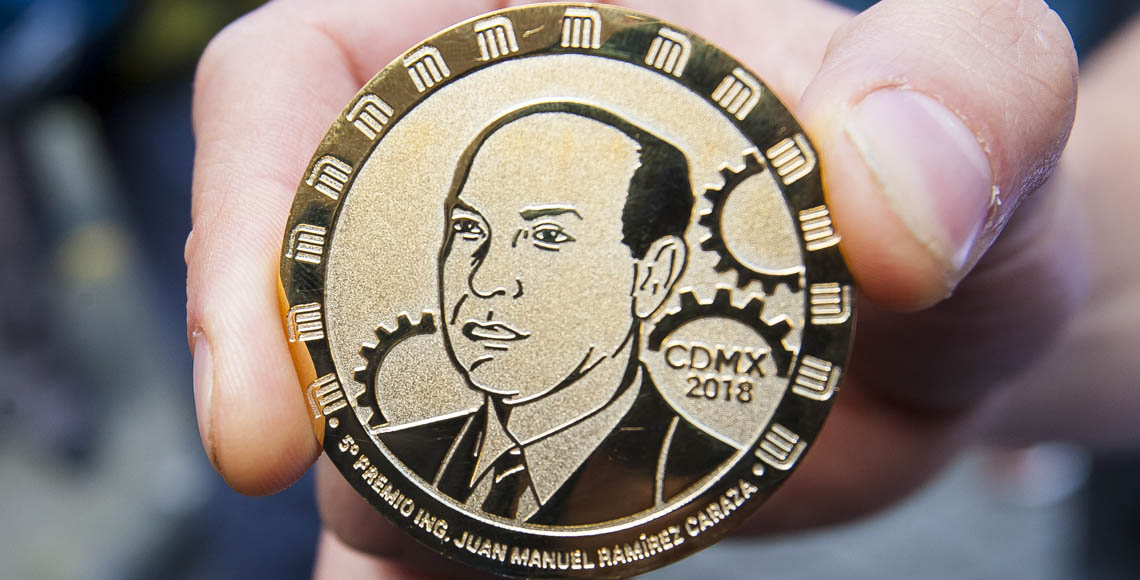
\includegraphics[width=0.6\textwidth]{capitulo_final/medalla}
    \caption{Medalla del quinto premio de innovación STCM}\label{fig:medalla}
\end{figure}

Se participó con un proyecto para utilizar una \hyperlink{abbr}{ConvNet} para
clasificar imágenes y detectar daños en los rieles en los que avanza el metro,
su título fue: 

\begin{quotation}
\textbf{Software de prueba basado en inteligencia artificial para la
    identificación y clasificación automática de daños superficiales en vías
    férreas del STC metro}
\end{quotation}

El trabajo representa un esfuerzo interinstitucional entre el Tecnológico
Nacional de México Campus Orizaba y el Instituto Politécnico Nacional de México.
En el proyecto participaron el autor de esta tesis y los aspirantes a doctor
Gerardo Bravo y Mario Guarneros, del grupo de tribología de la SEPI ESIME
Zacatenco. 

\subsection{Artículo JCR}

Finalmente, se colaboró en la publicación de un artículo JCR en la revistas
Multidisciplinary Digital Publishing Institute (\autoref{fig:mdpi}), con un
factor de impacto de 2.217. Este fue publicado en un volumen especial
Multi-Agent Systems 2019 que, como su nombre lo indica, se basó en la
presentación de artículos relacionados con sistemas multi-agente.

\begin{figure}[H]
    \centering
    
\includegraphics[width=0.6\textwidth]{capitulo_final/mdpi}
    \caption{MDPI}\label{fig:mdpi}
\end{figure}

El artículo fue recibido el día 14 de Octubre de 2019, aceptado el 6 de Noviembre y 
publicado el 15 de Noviembre de 2019.

Los autores y sus afiliaciones son las siguientes:

\begin{itemize}
    \item María del Rosario Pérez-Salazar -- Tecnológico Nacional de México /
    Instituto Tecnológico de Orizaba.
    \item Alberto Alfonso Aguilar-Lasserre -- Tecnológico Nacional de México /
    Instituto Tecnológico de Orizaba.
    \item Rubén Posada-Gómez -- Tecnológico Nacional de México /
    Instituto Tecnológico de Orizaba.
    \item Marco J. Del Moral-Argumedo -- Tecnológico Nacional de México /
    Instituto Tecnológico de Orizaba.
    \item José Carlos Hernández-González -- Tecnológico Nacional de México /
    Instituto Tecnológico de Orizaba. 
    \item Miguel Gastón Cedillo-Campos -- Instituto Mexicano del Transporte /
    Laboratorio Nacional de Logística y Sistemas de Transporte.
\end{itemize}

El título del artículo fue el siguiente:

\begin{quotation}
\textbf{An Agent-Based Model Driven Decision Support System for Reactive
    Aggregate Production Scheduling in the Green Coffee Supply Chain}
\end{quotation}

El abstract se muestra a continuación:

\begin{quotation}
\emph{Abstract: The aim of this paper is to contribute to the thread of research
regarding the need for logistic systems for planning and scheduling/rescheduling
within the agro-industry. To this end, an agent-based model driven decision
support system for the agri-food supply chain is presented. Inputs in this
research are taken from a case example of a Mexican green coffee supply chain.
In this context, the decision support agent serves the purposes of deriving
useful knowledge to accomplish (i) the decision regarding the estimation of
Cherry coffee yield obtained at the coffee plantation, and the Parchment coffee
sample verification decision, using fuzzy logic involving an inference engine
with IF-THEN type rules; (ii) the production plan establishment decision, using
a decision-making rule approach based upon the coupling of IF-THEN fuzzy
inference rules and equation-based representation by means of mixed integer
programming with the aim to maximize customer service level; and (iii) the
production plan update decision using mathematical equations once the customer
service level falls below the expected level. Three scenarios of demand patterns
were considered to conduct the experiments: increasing, unimodal and decreasing.
We found that the input inventory and output inventory vary similar over time
for the unimodal demand pattern, not the case for both the increasing and
decreasing demand patterns. For the decreasing demand pattern, ten tardy orders
for the initial production schedule, an 88\% service level, and nineteen tardy
orders from the estimated production results, a 77\% service level. This value
falls below the expected level. Consequently, the updated aggregate production
schedule resulted in ten tardy orders and an 88\% service level.}
\end{quotation}

La colaboración para la realización del artículo se basó en la optimización del
proceso de simulación en software mediante la traducción del modelo de lógica
difusa escrito en Matlab a lenguaje Python. Posteriormente se integró el modelo
traducido al software AnyLogic para usarse dentro de las
simulaciones. El resultado de esto fue una reducción considerable del tiempo de
simulación, de días u horas a minutos y segundos.